%%%%%%%%%%%%%%%%%%%%%%%%%%%%%%%%%%%%%%%%%%%%%%%%%%%%%%%%%%%%%%%%%%%%%%%%%%%%%%%%
%2345678901234567890123456789012345678901234567890123456789012345678901234567890
%        1         2         3         4         5         6         7         8

\documentclass[a4, 10 pt, conference]{ieeeconf}  % Comment this line out if you need a4paper

%\documentclass[a4paper, 10pt, conference]{ieeeconf}      % Use this line for a4 paper

\IEEEoverridecommandlockouts                              % This command is only needed if 
                                                          % you want to use the \thanks command

\overrideIEEEmargins                                      % Needed to meet printer requirements.

% See the \addtolength command later in the file to balance the column lengths
% on the last page of the document

% The following packages can be found on http:\\www.ctan.org
%\usepackage{graphics} % for pdf, bitmapped graphics files
%\usepackage{epsfig} % for postscript graphics files
%\usepackage{mathptmx} % assumes new font selection scheme installed
%\usepackage{times} % assumes new font selection scheme installed
%\usepackage{amsmath} % assumes amsmath package installed
%\usepackage{amssymb}  % assumes amsmath package installed
\usepackage{multicol}
\usepackage{tcolorbox}
\usepackage{cuted,tcolorbox,lipsum}
\usepackage{xcolor}
\usepackage{amsmath}

\title{\LARGE \bf
Introduction to Machine Learning (SS 2025)\\ Programming Project
\vspace{-3em}
}


%\author{Someone Anyone$^{1}$ and Xiang Zhang$^{2}$% <-this % stops a space
%}


\begin{document}


\maketitle
\vspace{-3em}
\thispagestyle{empty}
\pagestyle{empty}

\begin{strip}
\begin{tcolorbox}[
size=tight,
colback=white,
boxrule=0.2mm,
left=3mm,right=3mm, top=3mm, bottom=1mm
]
{\begin{multicols}{3}% replace 3 with 2 for 2 authors.

\textbf{Author 1}       \\
Last name:    Schweigl    \\  % Enter first name
First name:   Dominik    \\  % Enter first name
Matrikel Nr.: 12243381              \\  % Enter Matrikel number

\columnbreak

\textbf{Author 2}       \\
Last name:    Schöpf          \\  % Enter first name
First name:   Emanuel          \\  % Enter first name
Matrikel Nr.:               \\  % Enter Matrikel number

\columnbreak

% only four three person team
% \textbf{Author 3}       \\
% Last name:              \\  % Enter first name
% First name:             \\  % Enter first name
% Matrikel Nr.:               \\  % Enter Matrikel number

\end{multicols}}
\end{tcolorbox}
\end{strip}

%%%%%%%%%%%%%%%%%%%%%%%%%%%%%%%%%%%%%%%%%%%%%%%%%%%%%%%%%%%%%%%%%%%%%%%%%%%%%%%%

\section{Introduction}
\label{sec:intro}

For this report the task consists of classifying images of sign language hand gestures.
The dataset contains a total of 9680 instances of hands in a 128 x 128 pixel grayscale format.
Hence, this is a multilabel classification task, where each image corresponds to a
sign of the digits 0 to 9 and the letters a to z, totaling 36 classes.

The dataset is considerably imbalanced with the frequency for each sign ranging from
1.07\% to 5.78\%. 9 of the classes have frequencey of 5.78\%, 6 classes have 
frequency of 2.89\%, and the rest has ~1.50\% frequency.

\section{Implementation / ML Process}
\label{sec:methods}

The methods chosen for this task are a convolutional neural network (CNN), as
well as a multilabel support-vector-machine (SVM) classifier.

\subsection{Data preprocessing}
\label{subsec:preprocessing}

In order to avoid the machine learning methods not account well for minority classes or
learning wrong sign distributions or ignore minority classes and always predict the majority class
and misleading metrics like 90\% overall precision but 0\% recall for minority classes, 
the dataset was balanced by augmenting the instances of the minority classes.
The data was augmented using horizontal mirroring as well as 90\textdegree/$-90$\textdegree rotation based 
on how much augmentation was needed per class. The result is a dataset consisting
of 18056 instances with frequencies in the range of 2.48\% to 3.10\%. 

For the CNN it was found that more data was needed to increase the accuracy of the model
above 87\%. Therefore a dynamic data loader was implemented, which increases the 
dataset size by a specified factor using random augmentation of 15\textdegree rotation, 
horizontal mirroring, and random scaling between 80\% to 100\%. For the following 
a factor of 2 was used resulting in a dataset of 36112 instances with unchanged frequencies.

For the SVM classifier it was found necessary to scale the image values by $\frac{1}{255}$
to obtain features in the range $[0,1]$ for numerical stability. For values in the range $[0,255]$
the values for the radial basis function kernel $K(\mathbf{x}, \mathbf{x}') = \exp\left(-\gamma \|\mathbf{x} - \mathbf{x}'\|^2\right)$
 become very small, while linear and polynomial kernels $K(\mathbf{x}, \mathbf{x}') = \left(\mathbf{x}^\top \mathbf{x}' + c\right)^d$ become
extremely large, both resulting in issues during training with bad gradients and overflow.
Furthermore, it was found that it is not feasible for SVMs to work with high dimensional inputs
like our image dataset. Hence, PCA preprocessing with 200 components was applied to the images for the 
SVM classifier in order to retain 90\% explained variance.

\subsection{Classifier architecture}
\label{subsec:architecture}

A convolutional neural network was chosen because it is well-suited for image data. Unlike standard neural networks, CNNs use local receptive fields, which focus on small regions of the image at a time. This allows the network to capture spatial patterns and relationships between neighboring pixels more effectively.

Convolutional neural networks (CNNs) typically consist of convolutional layers at the beginning and fully connected layers at the end. The convolutional layers extract increasingly complex features from the input image, by applying small filters, called kernels, that slide over the input image. Each kernel detects specific local patterns such as edges, textures, or shapes by computing weighted sums of pixel values within its receptive field. As training progresses, the network learns kernels that extract features relevant to the classification task.

Pooling layers in between the convolutional layers progressively reduce the spatial dimensions of the convolutional feature maps (channels), which lowers the computational cost and the number of parameters in the network. In addition, pooling contributes to the increasing abstraction of features by summarizing local regions and increasing the receptive field. This makes the model more robust to small translations and distortions in the input. Max pooling, which selects the maximum value within each region, is the most commonly used pooling technique.

Fully connected layers are used at the end of CNNs to aggregate high-level features learned by the convolutional layers and map them to the output classes. They enable the network to learn complex, non-linear combinations of features and perform the final classification or regression task.

The chosen architecture of the CNN classifier consists of three convolutional layers followed by two fully connected layers, with the second producing the final class scores. Given the 128\texttimes128 input size, a single convolutional layer would be insufficient to extract meaningful hierarchical features. By stacking three convolutional layers, the model can progressively learn low-level patterns (such as edges), mid-level structures (like shapes), and higher-level abstractions relevant to classification. Each convolutional block is followed by 2\texttimes2 max pooling. The first fully connected layer processes the extracted features, while the second maps them to the 36 output classes.
The CNN is implemented using PyTorch. Figure 1 shows the chosen neural network architecture.

\begin{figure*}[htbp]
    \centering
    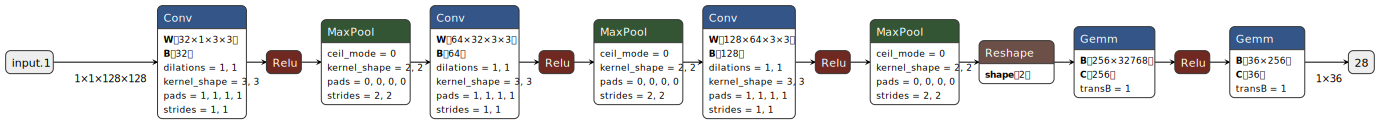
\includegraphics[width=\textwidth]{../images/sign_lang_model.onnx.png}
    \caption{Architecture of the CNN classifier. The CNN consists of 3 convolutional layers with 32, 64, and 128 channels respectively with ReLU activation function and 2 x 2 Pooling Layers. The Reshape layer converts the tensors of the convolutional layers to a 1 dimensional vector for the Linear (GeMM - General matrix multiplication) layers}
    \label{fig:cnn}
\end{figure*}

The support vector machine consists of an ensemble of support vector classifiers and is implemented using scikit-learns support vector classifier \texttt{sklearn.svm.SVC}. 
The SVM architecture was chosen as it focuses on maximizing the soft margin between classes. This makes it more robust to outliers and irrelevant features, which is especially beneficial when working with high-dimensional input such as PCA-transformed image data. Additionally, SVMs can achieve better generalization than logistic regression in cases where classes are not linearly separable, thanks to the ability to incorporate nonlinear kernels.

The support vector classifier works by finding the optimal hyperplane that separates the two classes while maximizing the margin between them. The margin is defined by the closest data points from each class, known as support vectors. By maximizing this margin, the classifier aims to achieve better generalization and robustness to small variations in the data. To account for noisy data and outliers, the margin can be made soft, allowing some misclassifications in exchange for better generalization.

Different kernel functions can be used in support vector machines to transform the input data into a higher-dimensional space, enabling the model to find a linear separation even when the original data is not linearly separable. The linear kernel is used when the data is already well separated in its original form, while the polynomial and radial basis function (RBF) kernels allow for more flexible, nonlinear decision boundaries by implicitly mapping the data to higher dimensions. This kernel trick enables SVMs to capture complex relationships between data points without explicitly computing the high-dimensional transformation, making them powerful for classification tasks with overlapping or curved class boundaries.

To extend binary support vector classifiers to multi-class classification, strategies such as one-vs-rest (OvR) and one-vs-one (OvO) are applied. In the one-vs-rest approach, a separate classifier is trained for each class to distinguish it from all other classes, and the classifier with the highest output score is selected for prediction. In the one-vs-one approach, a binary classifier is trained for every pair of classes, resulting in 
$\frac{K*(K-1)}{2}$ classifiers for $K$ classes. The final prediction is made by majority voting among the pairwise classifiers. Scikit-learn automatically handles this multi-class extension, allowing the ensemble of support vector classifiers to function as a single unified SVM across all 36 sign language classes.

The hinge loss is the loss function used by Support Vector Machines (SVMs). It encourages not only correct classification but also ensures that predictions are made with a sufficient margin between classes. Unlike log-loss, which is used by logistic regression and penalizes all misclassified points regardless of how far they are from the decision boundary, hinge loss penalizes predictions that lie within the margin or are misclassified. In addition, Hinge loss penalizes incorrect predictions linearly, making SVMs less sensitive to extreme outliers, unlike log-loss, which increases exponentially and overemphasizes such points.
The hinge loss for a sample $(\mathbf{x}, y)$, where $y \in \{-1, +1\}$, is defined as:
\[
\mathcal{L}_{hinge} = \max(0, 1 - y \cdot f(\mathbf{x}))
\]
where $f(\mathbf{x}) = \mathbf{w}^\top \mathbf{x} + b$ is the raw output of the classifier.
The log-loss (binary cross-entropy) for a sample $(\mathbf{x}, y)$, where $y \in \{0, 1\}$ and $\hat{y} = \sigma(f(\mathbf{x}))$ is the predicted probability, is defined as:
\[
\mathcal{L}_{log} = - \log(\sigma(y \cdot f(x)))
\]
where $\sigma(z) = \frac{1}{1 + e^{-z}}$ is the sigmoid function applied to the model output $f(\mathbf{x}) = \mathbf{w}^\top \mathbf{x} + b$.

It was decided against the use of k-Nearest Neighbors (k-NN) as it comes at a high
computational cost at inference since the test image to all training samples. In addition, 
decision trees and random forests were not implemented due to the large number of features, 
which likely makes them unsuitable as they only decide on a single feature at a time. Even though
these methods might produce acceptable results combined with feature extraction like PCA, they
were estimated to yield subpar performance. The use of an auto encoder was also hypothesized,
but it seemed too similar to the CNN architecture for this report. 

\subsection{Hyperparameters}
\label{subsec:hyperparameters}

The hyperparameter optimization was realized with random search. For each 
hyperparameter a numerical interval $[a, b]$ or a discrete set of choices $\{c,d,e,...\}$ 
was defined. Across 60 trials per classifier hyperparameters are uniformly sampled according
to the defined bounds, which are used to train a model on the dataset. The model is
evaluated using validation set and the best set of hyperparameters is selected
based on the resulting models performance.
For The Hyperparameter optimization of the CNN classifier the maximum training epochs
were set to 10 and it was performed on the dataset without additional augmentation due 
to time constraints. 

For the CNN classifier, random search was performed with a maximum of 40 training epochs. 
Early stopping was applied with a patience of 5 epochs, requiring a minimum improvement in 
validation loss of 0.01. Additionally, if validation accuracy did not reach at least 40\% by 
epoch 10, training was stopped early. PyTorchs \texttt{Adam} optimizer was used with default
parameters except learning rate. The search optimized across batch size $B$, learning rate
$l_R$ sampled from log-scale to bias small learning rates, kernel size $k$, number of convolutional channels $C_c$, linear layer size $n_h$, dropout
rate $d$, and activation function $f_A$. The number of convolutional layers was fixed to 3
and 1 hidden linear layer as seen in Figure~\ref{fig:cnn}. Table~\ref{fig:hyperparameter_selection} 
shows the search bounds and the final hyperparameters that achieved the best performance.

For the SVM classifier scikit-learns support vector classifier sklearn.svm.SVC was used.
The choice of the multi-class decision scheme OvO and OvR as well as the kernel function, 
the regularization parameter $C$, the kernel coefficient $\gamma$, and for the 
polynomial kernel the degree $d$ and the bias term $coef0$ were examined. The search bounds for these
hyperparameters as well as the final choice are depicted in Table~\ref{fig:hyperparameter_selection}.

\renewcommand{\arraystretch}{1.2}
\begin{table*}[htbp]
  \centering
  \begin{tabular}{|l|c|c|c|c|c|c|c|}
    \hline
    \multicolumn{8}{|l|}{CNN} \\
    \hline
    & $B$ & $l_R$ & $k$ & $n_h$ & $C_c$ & $d$ & $f_A$ \\
    \hline
    Bounds & $[8,128]$ & $[0.0001, 0.01]$ & $\{\text{3\texttimes3}, \text{5\texttimes5}\}$ & $[128,384]$ & $\{[16,32,64],[32,64,128],[48,96,192]\}$ & $[0.2,0.5]$ & $\{\text{ReLU}, \text{Sigmoid}\}$ \\
    Selection & 64 & 0.000218 & 5\texttimes5 & 382 & [32, 64, 128] & 0.2026 & ReLU\\
    \hline
    \multicolumn{8}{|l|}{SVM} \\
    \hline
    & $C$ & $\gamma$ & $d$ & coef0 & Kernel & \multicolumn{2}{c|}{multi-class decision scheme} \\
    \hline
    Bounds & [0.01, 1000] & [0.0001, 0.1] & [2, 4] & [0, 1] & \{Linear, Poly, RBF\} & \multicolumn{2}{c|}{\{OvO, OvR\}} \\
    Selection & 6 & 0.01 & 3 & 1 & Poly & \multicolumn{2}{c|}{OvO} \\
    \hline
  \end{tabular}
  \caption{Hyperparameter Selection for the CNN and SVM classifier.}
  \label{fig:hyperparameter_selection}
\end{table*}

\section{Results}
\label{sec:results}

The CNN classifier yiels significantly better results than the SVM classifier.
The final accuracies are shown in Table~\ref{tab:classifier_accuracy}.


\begin{table}[h]
  \centering
  \begin{tabular}{|l|c|c|}
    \hline
    & Train set & Validation set\\
    \hline
    CNN & 98.89\% & 98.56\% \\
    SVM & 100.00\% & 89.48\% \\
    \hline
  \end{tabular}
  \caption{Final classifier accuracy on training and validation.}
  \label{tab:classifier_accuracy}
\end{table}

The majority of remaining inaccuracy for both classifiers stem from a small set of similar
looking sign pairs, namely (O,0), (V,2), (W,6), and (M,N). This is clearly visible
in their respective confusion matrices shown in Figure~\ref{fig:cm}. The SVM 
classifier shows small amounts of confusion across the whole set of classes,
which explains the significantly lower validation accuracy.

\begin{figure}[htb]
  \centering
  \includegraphics[width=\linewidth]{../images/cm_comparison.jpg}
  \caption{Confusion matrices for CNN and SVM classifiers with ommitted diagonal.}
  \label{fig:cm}
\end{figure}

When plotting the per-class precision and accuracy values for the CNN classifier,
the pair wise confusion is seen by the duality between precision and recall of the 
respective confused pairs. This is best seen in the class pair (V,2) in 
Figure~\ref{fig:class_precision_recall}. The high precision and low recall for
class 2 shows that the model is quite conservative to classify an instance as 2. 
The opposite is seen in class V, which is mostly confused with 2, as it has high
recall and low precision. In combination with the results of the confusion matrix
this leads to the conclusion that the model has a tendency to classify the sign 2
as the sign V.

\begin{figure}[htb]
  \centering
  \includegraphics[width=\linewidth]{../images/class_accuracy_cnn.jpg}
  \caption{Per-class precision and recall of CNN classifier.}
  \label{fig:class_precision_recall}
\end{figure}

\section{Discussion}
\label{sec:discuss}

Initially, it was attempted to use the SVM classifier on the unprocessed image input
without normalization of pixel values and feature extraction. This led to no convergence
and the training had to be interrupted after a full day of training without result. While
SVMs can work for small image input like the MNIST datasets 28 x 28 images, it does not
scale to 128 x 128 images. It seems as the achieved results are already optimal for the 
SVM classifier architecture and are already over the model size requirements for this report.
The efforts to decrease the model size from the initial 110 MB by using the OvR strategy 
and polynomial kernels instead of rbf kernels for better compressibility and reduce the number of PCA components from 500
to 200, which lowered the explained variance from 95\% to 90\%, the model size was able to fit in 
the limit of 50 MB for this task. Surprisingly, these optimizations did not hurt the model performance.
Another promising approach would be to use the SVM classifier on image features extracted 
by an auto encoder instead of PCA.

Further improvements to the CNN classifier could likely be achieved by expanding the dataset and 
applying more extensive data augmentation. These factors appear to have been the most critical contributors to the CNN's 
improved performance, as the initial grid search on the unaugmented dataset did not reveal any consistently optimal 
hyperparameters. Class balancing and data augmentation were key in boosting classification accuracy. Initially, the CNN 
completely ignored minority classes, leading to 0\% recall for class W, with all W instances misclassified as class 6. 
This issue was addressed through targeted data augmentation for class balancing, as described in Section~\ref{subsec:preprocessing}. 
Following this augmentation, a second round of random search was conducted, which revealed clearer trends and distinctions 
in the effectiveness of different hyperparameter combinations.

{\color{blue}
\begin{itemize}
	\item Analyze the results presented in the report (comment on what contributed to the good or bad results). If your method does not work well, try to analyze why this is the case.
	\item Describe very briefly what you tried but did not keep for your final implementation (e.g. things you tried but that did not work, discarded ideas, etc.).
	\item How could you try to improve your results? What else would you want to try?

\end{itemize}
}

\section{Conclusion}
\label{sec:con}

The final CNN classifier was trained for 60 epochs on the entire training 
dataset and achieved a strong test dataset accuracy of x\%. In comparison, 
the SVM classifier reached a respectable y\%. While SVMs can be a viable 
alternative to CNNs for small multi-label classification tasks -- especially 
those involving few classes, small image sizes, and moderate amounts of 
data such as the MNIST dataset -- they do not scale as effectively as CNNs 
to larger images with many classes. This limitation persists even after 
dimensionality reduction with PCA, whereas learning compact representations 
with a convolutional autoencoder may provide feature spaces in which SVMs remain competitive.


{\color{blue}

  \begin{itemize}
  \item Finally, describe the test-set performance you achieved. Do not
    optimize your method based on the test set performance!
  \item Write a 5-10 line paragraph describing the main takeaway of your project.
  \end{itemize}

}

%%%%%%%%%%%%%%%%%%%%%%%%%%%%%%%%%%%%%%%%%%%%%%%%%%%%%%%%%%%%%%%%%%%%%%%%%%%%%%%%



\end{document}
